% ============================================================
%  Object Detection with OpenCV: From Classical to Deep Learning
%  LaTeX Beamer Presentation — 40 Frames
% ============================================================
\documentclass[aspectratio=169]{beamer}
\usetheme{Madrid}
\usepackage{amsmath,amssymb,tikz,listings,xcolor,booktabs,pgfplots}
\usetikzlibrary{arrows.meta,positioning,shapes,calc,fit}
\pgfplotsset{compat=1.18}
\lstset{language=Python,basicstyle=\ttfamily\tiny,keywordstyle=\color{blue},
  commentstyle=\color{gray},breaklines=true,showstringspaces=false}

\definecolor{cvblue}{RGB}{0,90,160}
\definecolor{cvgreen}{RGB}{34,139,34}
\definecolor{cvred}{RGB}{180,30,30}
\definecolor{cvorange}{RGB}{220,120,0}
\definecolor{lightgray}{RGB}{230,230,230}

\setbeamercolor{structure}{fg=cvblue}
\setbeamercolor{frametitle}{bg=cvblue,fg=white}
\setbeamercolor{block title}{bg=cvblue,fg=white}

\title[Object Detection with OpenCV]{Object Detection with OpenCV:\\
  From Classical to Deep Learning}
\subtitle{A Comprehensive Technical Guide}
\author{OpenCV Documentation}
\institute{opencv.org}
\date{\today}

% ============================================================
\begin{document}

% ============================================================
% FRAME 1 — Title
% ============================================================
\begin{frame}
  \titlepage
  \begin{tikzpicture}[remember picture,overlay]
    \node[anchor=south east,xshift=-10pt,yshift=10pt] at (current page.south east)
      {\small \textcolor{gray}{Covering: Template Matching, Haar, HOG, YOLO, SSD, Faster R-CNN}};
  \end{tikzpicture}
\end{frame}

% ============================================================
% FRAME 2 — What is Object Detection?
% ============================================================
\begin{frame}{What is Object Detection?}
  \begin{columns}
    \column{0.55\textwidth}
    \begin{block}{Three Levels of Understanding}
      \begin{itemize}
        \item \textbf{Classification}: What is in the image?
        \item \textbf{Detection}: What is it \emph{and where}? (bounding box + label)
        \item \textbf{Segmentation}: Pixel-level mask per object
      \end{itemize}
    \end{block}
    \vspace{4pt}
    Object detection = Classification + Localisation
    \column{0.42\textwidth}
    \begin{tikzpicture}[scale=0.85,every node/.style={font=\tiny}]
      % Input image
      \draw[thick,fill=lightgray] (0,0) rectangle (3.2,2.4);
      \node at (1.6,1.2) {\includegraphics[width=0pt,height=0pt]{}};
      \node[font=\scriptsize] at (1.6,2.1) {Input Image};
      % Object inside
      \draw[very thick,cvred] (0.5,0.4) rectangle (2.7,1.8);
      \node[fill=cvred,text=white,font=\scriptsize,inner sep=2pt]
            at (1.6,1.8) {Cat 0.97};
      % Arrow down
      \draw[-{Latex},thick] (1.6,-0.05) -- (1.6,-0.55);
      \node[draw,fill=cvblue,text=white,rounded corners,font=\scriptsize,
            inner sep=3pt] at (1.6,-0.85) {Detector Output};
      % BBox label
      \node[font=\tiny,align=center] at (1.6,-1.4)
        {[x1, y1, x2, y2, class, conf]};
    \end{tikzpicture}
  \end{columns}
\end{frame}

% ============================================================
% FRAME 3 — OpenCV Detection Ecosystem
% ============================================================
\begin{frame}{OpenCV Detection Ecosystem Overview}
  \begin{center}
  \small
  \begin{tabular}{lllll}
    \toprule
    \textbf{Method} & \textbf{Type} & \textbf{Training} & \textbf{GPU} & \textbf{Best For}\\
    \midrule
    Template Matching   & Classical & None        & No  & Rigid templates\\
    Haar Cascades       & Classical & Pretrained  & No  & Faces, objects\\
    HOG + SVM           & Classical & Optional    & No  & Pedestrians\\
    Background Subtraction & Classical & None     & No  & Moving objects\\
    OpenCV DNN (YOLO)   & Deep Learn. & Needed    & Yes & General objects\\
    OpenCV DNN (SSD)    & Deep Learn. & Needed    & Yes & Edge devices\\
    Faster R-CNN (DNN)  & Deep Learn. & Needed    & Yes & High accuracy\\
    Custom ONNX (YOLOv8) & Deep Learn. & Full     & Yes & Custom classes\\
    \bottomrule
  \end{tabular}
  \end{center}
  \begin{block}{Key OpenCV Namespaces}
    \texttt{cv2} · \texttt{cv2.dnn} · \texttt{cv2.CascadeClassifier} ·
    \texttt{cv2.HOGDescriptor} · \texttt{cv2.createBackgroundSubtractorMOG2()}
  \end{block}
\end{frame}

% ============================================================
% FRAME 4 — IoU Definition
% ============================================================
\begin{frame}{Intersection over Union (IoU)}
  \begin{columns}
    \column{0.48\textwidth}
    \begin{block}{Definition}
      \[
        \text{IoU} = \frac{|A \cap B|}{|A \cup B|}
                   = \frac{\text{Intersection Area}}{\text{Union Area}}
      \]
    \end{block}
    \begin{itemize}
      \item \textbf{IoU = 1.0}: perfect overlap
      \item \textbf{IoU $\geq$ 0.5}: commonly used threshold
      \item Used in NMS, mAP computation, anchor matching
    \end{itemize}
    \column{0.48\textwidth}
    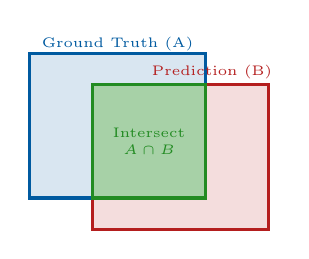
\begin{tikzpicture}[scale=0.8]
      % Ground truth box (blue)
      \draw[very thick,cvblue,fill=cvblue!15] (0,0.5) rectangle (2.8,2.8);
      \node[cvblue,font=\tiny] at (1.4,2.95) {Ground Truth (A)};
      % Predicted box (red)
      \draw[very thick,cvred,fill=cvred!15] (1.0,0) rectangle (3.8,2.3);
      \node[cvred,font=\tiny] at (2.9,2.5) {Prediction (B)};
      % Intersection hatched
      \begin{scope}
        \clip (0,0.5) rectangle (2.8,2.8);
        \clip (1.0,0) rectangle (3.8,2.3);
        \fill[cvgreen!40] (1.0,0.5) rectangle (2.8,2.3);
      \end{scope}
      \draw[very thick,cvgreen] (1.0,0.5) rectangle (2.8,2.3);
      \node[cvgreen,font=\tiny,align=center] at (1.9,1.4)
            {Intersect\\$A\cap B$};
    \end{tikzpicture}
  \end{columns}
\end{frame}

% ============================================================
% PART 2 — CLASSICAL METHODS
% ============================================================

% FRAME 5 — Template Matching
\begin{frame}{Template Matching — Algorithm}
  \begin{columns}
    \column{0.52\textwidth}
    \begin{block}{Algorithm}
      Slide template $T(w\times h)$ over image $I$ and compute a similarity
      score at every position $(x,y)$:
      \[
        R(x,y) = \text{metric}(I[y:y{+}h,\, x:x{+}w],\; T)
      \]
      Peak of $R$ gives best match location.
    \end{block}
    \vspace{4pt}
    \begin{tabular}{ll}
      \toprule
      \textbf{Flag} & \textbf{Method}\\
      \midrule
      \texttt{TM\_SQDIFF}       & Sum of squared diff.\\
      \texttt{TM\_SQDIFF\_NORMED} & Normalised SSD\\
      \texttt{TM\_CCORR}        & Cross-correlation\\
      \texttt{TM\_CCORR\_NORMED} & Normalised CC\\
      \texttt{TM\_CCOEFF}       & Correlation coeff.\\
      \texttt{TM\_CCOEFF\_NORMED} & \textbf{Best general use}\\
      \bottomrule
    \end{tabular}
    \column{0.44\textwidth}
    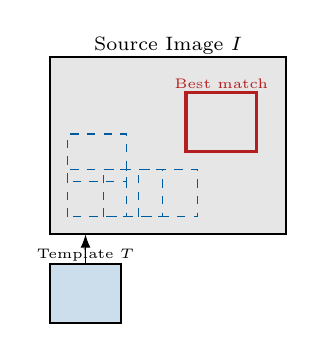
\begin{tikzpicture}[scale=0.75,every node/.style={font=\tiny}]
      % Source image
      \draw[fill=lightgray,thick] (0,0) rectangle (4,3);
      \node[font=\scriptsize] at (2,3.2) {Source Image $I$};
      % Sliding window
      \foreach \x/\y in {0.3/0.3, 0.9/0.3, 1.5/0.3, 0.3/0.9}{
        \draw[cvblue,thin,dashed] (\x,\y) rectangle ++(1.0,0.8);
      }
      % Template match highlight
      \draw[cvred,very thick] (2.3,1.4) rectangle ++(1.2,1.0);
      \node[cvred] at (2.9,2.55) {Best match};
      % Template
      \draw[fill=cvblue!20,thick] (0,-1.5) rectangle (1.2,-0.5);
      \node at (0.6,-0.35) {Template $T$};
      % Arrow
      \draw[-{Latex}] (0.6,-0.5) -- (0.6,0);
    \end{tikzpicture}
  \end{columns}
\end{frame}

% FRAME 6 — Template Matching Code
\begin{frame}[fragile]{Template Matching — Code}
\begin{lstlisting}
import cv2
import numpy as np

# Load source and template
img  = cv2.imread('scene.jpg',  cv2.IMREAD_GRAYSCALE)
tmpl = cv2.imread('template.jpg', cv2.IMREAD_GRAYSCALE)
h, w = tmpl.shape

# Run matching
result = cv2.matchTemplate(img, tmpl, cv2.TM_CCOEFF_NORMED)

# Find best match and apply threshold
threshold = 0.8
loc = np.where(result >= threshold)
min_val, max_val, min_loc, max_loc = cv2.minMaxLoc(result)

# Draw bounding box for best match (TM_CCOEFF_NORMED: use max_loc)
top_left  = max_loc
bot_right = (top_left[0] + w, top_left[1] + h)
cv2.rectangle(img, top_left, bot_right, 255, 2)

# Multi-match: iterate over threshold hits
for pt in zip(*loc[::-1]):
    cv2.rectangle(img, pt, (pt[0]+w, pt[1]+h), (0,0,255), 1)

cv2.imshow('Template Matching', img)
cv2.waitKey(0)
\end{lstlisting}
\begin{block}{Limitations}
  Sensitive to scale changes, rotation, and lighting variation.
\end{block}
\end{frame}

% FRAME 7 — Haar Cascades
\begin{frame}{Haar Cascades — Viola-Jones Framework}
  \begin{columns}
    \column{0.5\textwidth}
    \begin{block}{Key Innovations (Viola \& Jones, 2001)}
      \begin{enumerate}
        \item \textbf{Integral images} — $O(1)$ rectangle sum lookups
        \item \textbf{Haar-like features} — fast edge/line detectors
        \item \textbf{AdaBoost} — select best $N$ features from 160 000+
        \item \textbf{Cascade} — early rejection of non-face windows
      \end{enumerate}
    \end{block}
    \column{0.46\textwidth}
    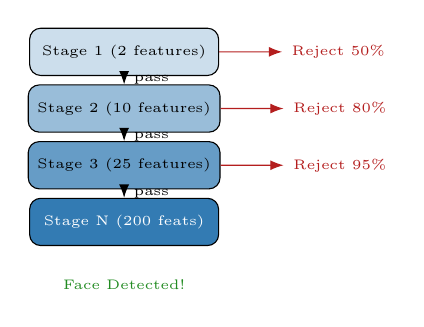
\begin{tikzpicture}[scale=0.72,every node/.style={font=\tiny}]
      \node[draw,fill=cvblue!20,rounded corners,minimum width=2.4cm,minimum height=0.6cm]
            (s1) at (0,3) {Stage 1 (2 features)};
      \node[draw,fill=cvblue!40,rounded corners,minimum width=2.4cm,minimum height=0.6cm]
            (s2) at (0,2) {Stage 2 (10 features)};
      \node[draw,fill=cvblue!60,rounded corners,minimum width=2.4cm,minimum height=0.6cm]
            (s3) at (0,1) {Stage 3 (25 features)};
      \node[draw,fill=cvblue!80,text=white,rounded corners,minimum width=2.4cm,minimum height=0.6cm]
            (sn) at (0,0) {Stage N (200 feats)};
      \draw[-{Latex}] (s1)--(s2) node[midway,right]{pass};
      \draw[-{Latex}] (s2)--(s3) node[midway,right]{pass};
      \draw[-{Latex}] (s3)--(sn) node[midway,right]{pass};
      \node[cvred,right=0.8cm of s1,font=\tiny] (r1) {Reject 50\%};
      \node[cvred,right=0.8cm of s2,font=\tiny] (r2) {Reject 80\%};
      \node[cvred,right=0.8cm of s3,font=\tiny] (r3) {Reject 95\%};
      \draw[cvred,-{Latex}] (s1.east)--(r1.west);
      \draw[cvred,-{Latex}] (s2.east)--(r2.west);
      \draw[cvred,-{Latex}] (s3.east)--(r3.west);
      \node[cvgreen,below=0.3cm of sn] {Face Detected!};
    \end{tikzpicture}
  \end{columns}
\end{frame}

% FRAME 8 — Haar Features Diagram
\begin{frame}{Haar-Like Features}
  \begin{center}
  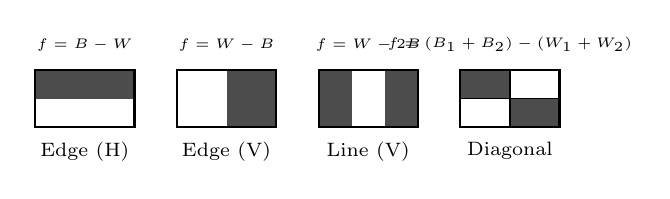
\begin{tikzpicture}[scale=0.9,every node/.style={font=\scriptsize}]
    % Edge feature horizontal
    \begin{scope}[xshift=0cm]
      \draw[thick] (0,0) rectangle (1.4,0.8);
      \fill[black!70] (0,0.4) rectangle (1.4,0.8);
      \fill[white] (0,0) rectangle (1.4,0.4);
      \draw[thick] (0,0) rectangle (1.4,0.8);
      \node[below=2pt] at (0.7,0) {Edge (H)};
    \end{scope}
    % Edge feature vertical
    \begin{scope}[xshift=2cm]
      \fill[white] (0,0) rectangle (0.7,0.8);
      \fill[black!70] (0.7,0) rectangle (1.4,0.8);
      \draw[thick] (0,0) rectangle (1.4,0.8);
      \node[below=2pt] at (0.7,0) {Edge (V)};
    \end{scope}
    % Line feature
    \begin{scope}[xshift=4cm]
      \fill[black!70] (0,0) rectangle (0.47,0.8);
      \fill[white] (0.47,0) rectangle (0.93,0.8);
      \fill[black!70] (0.93,0) rectangle (1.4,0.8);
      \draw[thick] (0,0) rectangle (1.4,0.8);
      \node[below=2pt] at (0.7,0) {Line (V)};
    \end{scope}
    % 4-rectangle feature
    \begin{scope}[xshift=6cm]
      \fill[black!70] (0,0.4) rectangle (0.7,0.8);
      \fill[white]    (0.7,0.4) rectangle (1.4,0.8);
      \fill[white]    (0,0) rectangle (0.7,0.4);
      \fill[black!70] (0.7,0) rectangle (1.4,0.4);
      \draw[thick] (0,0) rectangle (1.4,0.8);
      \draw[thin]  (0,0.4)--(1.4,0.4);
      \draw[thin]  (0.7,0)--(0.7,0.8);
      \node[below=2pt] at (0.7,0) {Diagonal};
    \end{scope}
    % Labels
    \node[above=2pt,font=\tiny\itshape] at (0.7,0.85) {$f = B - W$};
    \node[above=2pt,font=\tiny\itshape] at (2.7,0.85) {$f = W - B$};
    \node[above=2pt,font=\tiny\itshape] at (4.7,0.85) {$f = W - 2B$};
    \node[above=2pt,font=\tiny\itshape] at (6.7,0.85) {$f = (B_1+B_2)-(W_1+W_2)$};
  \end{tikzpicture}
  \end{center}
  \begin{block}{Feature Value}
    $f = \sum_{\text{white region}} - \sum_{\text{black region}}$, computed in $O(1)$
    using the \textbf{Integral Image}: $II(x,y) = \sum_{x'\le x,\,y'\le y} I(x',y')$
  \end{block}
\end{frame}

% FRAME 9 — Haar Cascades Code
\begin{frame}[fragile]{Haar Cascades — OpenCV Code}
\begin{lstlisting}
import cv2

# Load pretrained cascade
face_cascade = cv2.CascadeClassifier(
    cv2.data.haarcascades + 'haarcascade_frontalface_default.xml')
eye_cascade  = cv2.CascadeClassifier(
    cv2.data.haarcascades + 'haarcascade_eye.xml')

img  = cv2.imread('group.jpg')
gray = cv2.cvtColor(img, cv2.COLOR_BGR2GRAY)

# detectMultiScale parameters
faces = face_cascade.detectMultiScale(
    gray,
    scaleFactor=1.1,    # Image pyramid scale (1.05 slower/more accurate)
    minNeighbors=5,     # Min neighbours to retain detection
    minSize=(30, 30),   # Minimum object size in pixels
    flags=cv2.CASCADE_SCALE_IMAGE)

for (x, y, w, h) in faces:
    cv2.rectangle(img, (x,y), (x+w, y+h), (255,0,0), 2)
    roi_gray = gray[y:y+h, x:x+w]
    eyes = eye_cascade.detectMultiScale(roi_gray, 1.1, 3)
    for (ex, ey, ew, eh) in eyes:
        cv2.rectangle(img, (x+ex, y+ey), (x+ex+ew, y+ey+eh), (0,255,0), 2)
\end{lstlisting}
\small
\begin{tabular}{lll}
  \toprule
  \textbf{Param} & \textbf{Default} & \textbf{Effect}\\
  \midrule
  \texttt{scaleFactor}  & 1.1   & Pyramid step; lower = more scales checked\\
  \texttt{minNeighbors} & 3     & Higher = fewer false positives\\
  \texttt{minSize}      & (0,0) & Skip small detection windows\\
  \bottomrule
\end{tabular}
\end{frame}

% FRAME 10 — HOG Features
\begin{frame}{HOG Features — Histogram of Oriented Gradients}
  \begin{columns}
    \column{0.52\textwidth}
    \begin{block}{Dalal \& Triggs, 2005}
      \begin{enumerate}
        \item Compute image gradients: $G_x = I * [-1,0,1]$
        \item Magnitude: $|G| = \sqrt{G_x^2+G_y^2}$
        \item Orientation: $\theta = \arctan(G_y/G_x)$
        \item Bin orientations into 9-bin histogram per $8\times8$ cell
        \item Normalise over $2\times2$ block ($L2$-norm)
        \item Concatenate all block descriptors
      \end{enumerate}
    \end{block}
    \textbf{Descriptor size}: $64\times128$ window $\Rightarrow$ 3780-dim vector
    \column{0.44\textwidth}
    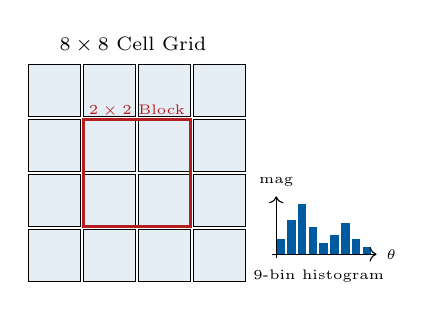
\begin{tikzpicture}[scale=0.7,every node/.style={font=\tiny}]
      % Cell grid
      \foreach \x in {0,1,2,3}{
        \foreach \y in {0,1,2,3}{
          \draw[fill=cvblue!10] (\x,\y) rectangle ++(.95,.95);
        }
      }
      \node[font=\scriptsize] at (1.9,4.3) {$8\times8$ Cell Grid};
      % Block outline
      \draw[cvred,very thick] (1,1) rectangle (2.95,2.95);
      \node[cvred] at (1.97,3.1) {$2\times2$ Block};
      % Histogram bars for one cell
      \begin{scope}[xshift=4.5cm,yshift=0.5cm,scale=0.7]
        \foreach \i/\h in {0/0.4, 1/0.9, 2/1.3, 3/0.7, 4/0.3, 5/0.5, 6/0.8, 7/0.4, 8/0.2}{
          \fill[cvblue] (\i*0.28,0) rectangle ++(.22,\h);
        }
        \draw[->] (-0.1,0) -- (2.6,0);
        \draw[->] (0,-0.1) -- (0,1.5);
        \node[right] at (2.6,0) {$\theta$};
        \node[above] at (0,1.5) {mag};
        \node[below] at (1.1,-0.15) {9-bin histogram};
      \end{scope}
    \end{tikzpicture}
  \end{columns}
\end{frame}

% FRAME 11 — HOG+SVM Pipeline
\begin{frame}{HOG+SVM Detection Pipeline}
  \begin{center}
  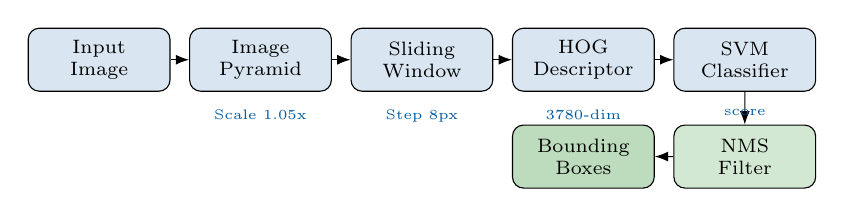
\begin{tikzpicture}[scale=0.82,every node/.style={font=\scriptsize},
      box/.style={draw,fill=cvblue!15,rounded corners,minimum width=1.8cm,
                  minimum height=0.8cm,align=center}]
    \node[box] (img) at (0,0)     {Input\\Image};
    \node[box] (pyr) at (2.5,0)   {Image\\Pyramid};
    \node[box] (win) at (5,0)     {Sliding\\Window};
    \node[box] (hog) at (7.5,0)   {HOG\\Descriptor};
    \node[box] (svm) at (10,0)    {SVM\\Classifier};
    \node[box,fill=cvgreen!20] (nms) at (10,-1.5) {NMS\\Filter};
    \node[box,fill=cvgreen!30] (out) at (7.5,-1.5) {Bounding\\Boxes};
    \draw[-{Latex}] (img)--(pyr);
    \draw[-{Latex}] (pyr)--(win);
    \draw[-{Latex}] (win)--(hog);
    \draw[-{Latex}] (hog)--(svm);
    \draw[-{Latex}] (svm)--(nms);
    \draw[-{Latex}] (nms)--(out);
    \node[font=\tiny,below=3pt of pyr,cvblue] {Scale 1.05x};
    \node[font=\tiny,below=3pt of win,cvblue] {Step 8px};
    \node[font=\tiny,below=3pt of hog,cvblue] {3780-dim};
    \node[font=\tiny,below=3pt of svm,cvblue] {score};
  \end{tikzpicture}
  \end{center}
  \begin{columns}
    \column{0.48\textwidth}
    \begin{lstlisting}[basicstyle=\ttfamily\scriptsize]
hog = cv2.HOGDescriptor()
hog.setSVMDetector(
  cv2.HOGDescriptor_getDefaultPeopleDetector())
rects, weights = hog.detectMultiScale(
    img, winStride=(8,8), padding=(8,8),
    scale=1.05)
    \end{lstlisting}
    \column{0.48\textwidth}
    \begin{itemize}
      \item \textbf{winStride}: overlap between windows
      \item \textbf{scale}: pyramid scale factor
      \item Pretrained SVM for pedestrian detection included
    \end{itemize}
  \end{columns}
\end{frame}

% FRAME 12 — Background Subtraction
\begin{frame}{Background Subtraction — MOG2}
  \begin{columns}
    \column{0.52\textwidth}
    \begin{block}{Gaussian Mixture Model per Pixel (Zivkovic, 2004)}
      Each pixel $p$ modelled as mixture of $K$ Gaussians:
      \[
        P(X_t) = \sum_{k=1}^{K} \omega_{k,t}\;\mathcal{N}(X_t;\,\mu_k,\,\sigma_k^2)
      \]
      Background = Gaussians with high weight $\omega$ and low variance $\sigma^2$.
    \end{block}
    \begin{itemize}
      \item Handles multi-modal backgrounds (waving trees)
      \item Automatically adapts over time
      \item Shadow detection built in
    \end{itemize}
    \column{0.44\textwidth}
    \begin{lstlisting}
import cv2
cap = cv2.VideoCapture('video.mp4')
mog2 = cv2.createBackgroundSubtractorMOG2(
    history=500,
    varThreshold=16,
    detectShadows=True)

while True:
    ret, frame = cap.read()
    if not ret: break
    fg_mask = mog2.apply(frame)
    # Remove shadows (127 -> 0)
    _, fg_mask = cv2.threshold(
        fg_mask, 200, 255,
        cv2.THRESH_BINARY)
    cv2.imshow('FG', fg_mask)
    if cv2.waitKey(30) == 27: break
    \end{lstlisting}
  \end{columns}
\end{frame}

% FRAME 13 — Contour Detection Pipeline
\begin{frame}[fragile]{Contour-Based Detection Pipeline}
  \begin{lstlisting}
import cv2
import numpy as np

img  = cv2.imread('objects.jpg')
gray = cv2.cvtColor(img, cv2.COLOR_BGR2GRAY)

# Preprocessing
blur  = cv2.GaussianBlur(gray, (5,5), 0)
edges = cv2.Canny(blur, 50, 150)          # or threshold + findContours

# Morphological operations to close gaps
kernel  = cv2.getStructuringElement(cv2.MORPH_RECT, (5,5))
dilated = cv2.dilate(edges, kernel, iterations=2)
closed  = cv2.morphologyEx(dilated, cv2.MORPH_CLOSE, kernel)

# Find and filter contours
contours, hierarchy = cv2.findContours(
    closed, cv2.RETR_EXTERNAL, cv2.CHAIN_APPROX_SIMPLE)

for cnt in contours:
    area = cv2.contourArea(cnt)
    if area < 500: continue                      # filter noise
    x, y, w, h = cv2.boundingRect(cnt)
    aspect = w / float(h)
    if 0.5 < aspect < 3.0:                       # shape filter
        cv2.rectangle(img, (x,y), (x+w,y+h), (0,255,0), 2)
        hull = cv2.convexHull(cnt)
        cv2.drawContours(img, [hull], -1, (0,0,255), 1)
  \end{lstlisting}
\end{frame}

% FRAME 14 — Non-Maximum Suppression
\begin{frame}{Non-Maximum Suppression (NMS)}
  \begin{columns}
    \column{0.5\textwidth}
    \begin{block}{Algorithm}
      \begin{enumerate}
        \item Sort boxes by confidence score (descending)
        \item Pick highest-score box $B_1$; add to output
        \item Remove all boxes with $\text{IoU}(B_1, B_i) > \tau$
        \item Repeat until no boxes remain
      \end{enumerate}
    \end{block}
    \[
      \text{Soft-NMS}: s_i = s_i \cdot e^{-\text{IoU}(B_1,B_i)^2/\sigma}
    \]
    OpenCV: \texttt{cv2.dnn.NMSBoxes(boxes, scores, score\_thresh, nms\_thresh)}
    \column{0.46\textwidth}
    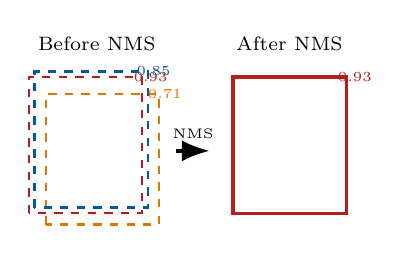
\begin{tikzpicture}[scale=0.72,every node/.style={font=\tiny}]
      % Before NMS
      \node[font=\scriptsize,above] at (1.2,3.1) {Before NMS};
      \draw[cvred,thick,dashed]   (0.0,0.4) rectangle (2.0,2.8);
      \draw[cvorange,thick,dashed](0.3,0.2) rectangle (2.3,2.5);
      \draw[cvblue,thick,dashed]  (0.1,0.5) rectangle (2.1,2.9);
      \node[cvred]   at (2.15,2.8) {0.93};
      \node[cvorange]at (2.4,2.5) {0.71};
      \node[cvblue]  at (2.2,2.9) {0.85};
      % Arrow
      \draw[-{Latex},ultra thick] (2.6,1.5) -- (3.2,1.5);
      \node[above,font=\tiny] at (2.9,1.55) {NMS};
      % After NMS
      \node[font=\scriptsize,above] at (4.6,3.1) {After NMS};
      \draw[cvred,very thick] (3.6,0.4) rectangle (5.6,2.8);
      \node[cvred] at (5.75,2.8) {0.93};
    \end{tikzpicture}
  \end{columns}
\end{frame}

% ============================================================
% PART 3 — DEEP LEARNING METHODS
% ============================================================

% FRAME 15 — OpenCV DNN Module
\begin{frame}{OpenCV DNN Module}
  \begin{columns}
    \column{0.5\textwidth}
    \begin{block}{Supported Frameworks}
      Caffe · TensorFlow · PyTorch (ONNX) · Darknet · TFLite · OpenVINO IR
    \end{block}
    \begin{block}{Core API}
      \begin{itemize}
        \item \texttt{cv2.dnn.readNet(weights, config)}
        \item \texttt{cv2.dnn.readNetFromONNX(path)}
        \item \texttt{cv2.dnn.blobFromImage(img, scale, size, mean, swapRB)}
        \item \texttt{net.setInput(blob)}
        \item \texttt{net.forward(layerNames)} $\rightarrow$ outputs
      \end{itemize}
    \end{block}
    \column{0.46\textwidth}
    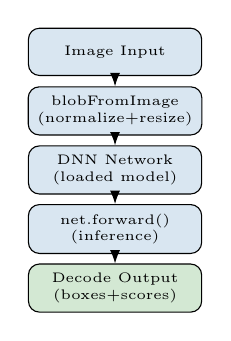
\begin{tikzpicture}[scale=0.75,every node/.style={font=\tiny},
        box/.style={draw,rounded corners,fill=cvblue!15,minimum width=2.2cm,
                    minimum height=0.6cm,align=center}]
      \node[box] (inp)  at (0,4)   {Image Input};
      \node[box] (blob) at (0,3)   {blobFromImage\\(normalize+resize)};
      \node[box] (net)  at (0,2)   {DNN Network\\(loaded model)};
      \node[box] (fwd)  at (0,1)   {net.forward()\\(inference)};
      \node[box,fill=cvgreen!20] (dec) at (0,0) {Decode Output\\(boxes+scores)};
      \foreach \a/\b in {inp/blob,blob/net,net/fwd,fwd/dec}{
        \draw[-{Latex}] (\a)--(\b);
      }
    \end{tikzpicture}
  \end{columns}
\end{frame}

% FRAME 16 — Detection Paradigms
\begin{frame}{Neural Network Detection Paradigms}
  \begin{columns}
    \column{0.48\textwidth}
    \begin{block}{Two-Stage (Faster R-CNN)}
      \begin{enumerate}
        \item \textbf{Stage 1}: Region Proposal Network (RPN) proposes $\sim$300 ROIs
        \item \textbf{Stage 2}: ROI-Pooling + classifier/regressor per region
      \end{enumerate}
      \textbf{Pros}: Higher accuracy \\
      \textbf{Cons}: Slower (5--10 fps on GPU)
    \end{block}
    \column{0.48\textwidth}
    \begin{block}{One-Stage (YOLO, SSD)}
      Single forward pass predicts \textbf{all} boxes simultaneously on a dense grid.\\[4pt]
      \textbf{Pros}: Real-time (30--200+ fps) \\
      \textbf{Cons}: Slightly lower accuracy on small objects
    \end{block}
  \end{columns}
  \vspace{6pt}
  \begin{center}
  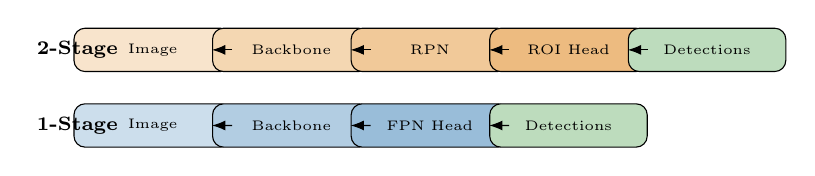
\begin{tikzpicture}[scale=0.8,every node/.style={font=\tiny},
      box/.style={draw,rounded corners,minimum width=2cm,minimum height=0.55cm,align=center}]
    % Two-stage
    \node[box,fill=cvorange!20] (img1) at (0,0) {Image};
    \node[box,fill=cvorange!30] (bb)   at (2.2,0) {Backbone};
    \node[box,fill=cvorange!40] (rpn)  at (4.4,0) {RPN};
    \node[box,fill=cvorange!50] (roi)  at (6.6,0) {ROI Head};
    \node[box,fill=cvgreen!30]  (out1) at (8.8,0) {Detections};
    \foreach \a/\b in {img1/bb,bb/rpn,rpn/roi,roi/out1}{\draw[-{Latex}](\a)--(\b);}
    \node[left,font=\scriptsize\bfseries] at (-0.4,0) {2-Stage};
    % One-stage
    \node[box,fill=cvblue!20] (img2) at (0,-1.2) {Image};
    \node[box,fill=cvblue!30] (bb2)  at (2.2,-1.2) {Backbone};
    \node[box,fill=cvblue!40] (fpn)  at (4.4,-1.2) {FPN Head};
    \node[box,fill=cvgreen!30](out2) at (6.6,-1.2) {Detections};
    \foreach \a/\b in {img2/bb2,bb2/fpn,fpn/out2}{\draw[-{Latex}](\a)--(\b);}
    \node[left,font=\scriptsize\bfseries] at (-0.4,-1.2) {1-Stage};
  \end{tikzpicture}
  \end{center}
\end{frame}

% FRAME 17 — YOLO Architecture
\begin{frame}{YOLO Architecture Overview}
  \begin{center}
  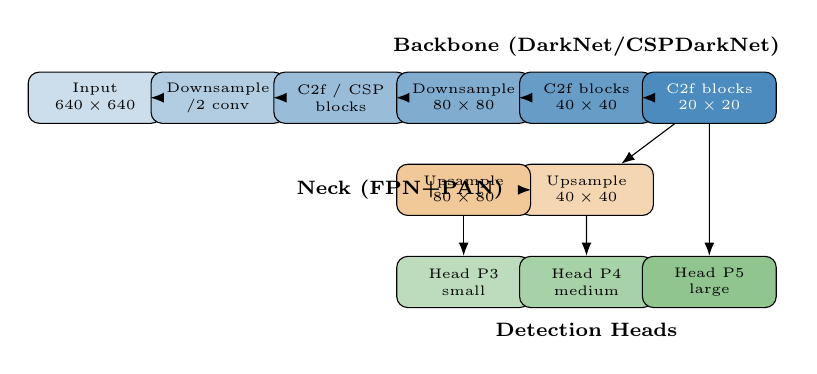
\begin{tikzpicture}[scale=0.78,every node/.style={font=\tiny},
      box/.style={draw,rounded corners,minimum width=1.7cm,minimum height=0.65cm,align=center}]
    % Backbone
    \node[box,fill=cvblue!20] (inp) at (0,0)   {Input\\$640\times640$};
    \node[box,fill=cvblue!30] (ds1) at (2,0)   {Downsample\\/2 conv};
    \node[box,fill=cvblue!40] (c2f) at (4,0)   {C2f / CSP\\blocks};
    \node[box,fill=cvblue!50] (ds2) at (6,0)   {Downsample\\$80\times80$};
    \node[box,fill=cvblue!60] (c2f2)at (8,0)   {C2f blocks\\$40\times40$};
    \node[box,fill=cvblue!70,text=white] (c2f3) at (10,0) {C2f blocks\\$20\times20$};
    % FPN
    \node[box,fill=cvorange!30] (up1) at (8,-1.5) {Upsample\\$40\times40$};
    \node[box,fill=cvorange!40] (up2) at (6,-1.5) {Upsample\\$80\times80$};
    % Heads
    \node[box,fill=cvgreen!30] (h1) at (6,-3)  {Head P3\\small};
    \node[box,fill=cvgreen!40] (h2) at (8,-3)  {Head P4\\medium};
    \node[box,fill=cvgreen!50] (h3) at (10,-3) {Head P5\\large};
    % Backbone path
    \foreach \a/\b in {inp/ds1,ds1/c2f,c2f/ds2,ds2/c2f2,c2f2/c2f3}{\draw[-{Latex}](\a)--(\b);}
    % FPN paths
    \draw[-{Latex}] (c2f3)--(up1);
    \draw[-{Latex}] (up1)--(up2);
    \draw[-{Latex}] (up2)--(h1);
    \draw[-{Latex}] (up1)--(h2);
    \draw[-{Latex}] (c2f3)--(h3);
    \node[font=\scriptsize\bfseries,above=2pt of c2f2] {Backbone (DarkNet/CSPDarkNet)};
    \node[font=\scriptsize\bfseries,left=2pt of up1] {Neck (FPN+PAN)};
    \node[font=\scriptsize\bfseries,below=2pt of h2] {Detection Heads};
  \end{tikzpicture}
  \end{center}
\end{frame}

% FRAME 18 — YOLO Grid and Anchors
\begin{frame}{YOLO Grid Cell Prediction and Anchor Boxes}
  \begin{columns}
    \column{0.5\textwidth}
    \begin{block}{Grid Cell Responsibility}
      If object centre falls in cell $(c_x, c_y)$, that cell predicts it.
      Each cell predicts $B$ boxes (one per anchor), each with:
      \begin{itemize}
        \item $t_x, t_y$: centre offset from cell
        \item $t_w, t_h$: log-scale dimension
        \item $t_o$: objectness score
        \item $p_1,\ldots,p_C$: class probabilities
      \end{itemize}
      Total output per cell: $B \times (5 + C)$
    \end{block}
    \column{0.46\textwidth}
    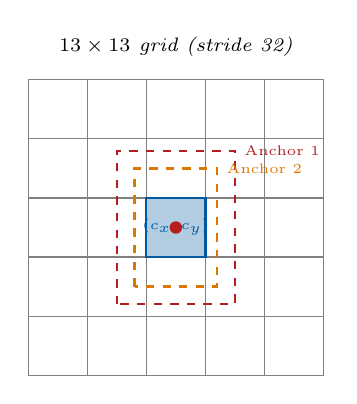
\begin{tikzpicture}[scale=0.75,every node/.style={font=\tiny}]
      % Grid
      \foreach \x in {0,...,4}{
        \foreach \y in {0,...,4}{
          \draw[gray,thin] (\x,\y) rectangle ++(1,1);
        }
      }
      % Highlighted cell
      \fill[cvblue!30] (2,2) rectangle (3,3);
      \draw[cvblue,thick] (2,2) rectangle (3,3);
      \node[cvblue] at (2.5,2.5) {$(c_x,c_y)$};
      % Anchor boxes
      \draw[cvred,thick,dashed]   (1.5,1.2) rectangle (3.5,3.8);
      \draw[cvorange,thick,dashed](1.8,1.5) rectangle (3.2,3.5);
      \node[cvred,right]   at (3.5,3.8) {Anchor 1};
      \node[cvorange,right]at (3.2,3.5) {Anchor 2};
      % Centre dot
      \fill[cvred] (2.5,2.5) circle (3pt);
      \node[font=\scriptsize\itshape,above=5pt] at (2.5,5) {$13\times13$ grid (stride 32)};
    \end{tikzpicture}
  \end{columns}
\end{frame}

% FRAME 19 — YOLO Output Decoding Math
\begin{frame}{YOLO Output Decoding Formulas}
  \begin{block}{Bounding Box Decoding (YOLOv3/v4)}
    \[
      b_x = \sigma(t_x) + c_x \qquad b_y = \sigma(t_y) + c_y
    \]
    \[
      b_w = p_w\, e^{t_w} \qquad b_h = p_h\, e^{t_h}
    \]
    \[
      \text{Objectness} = \sigma(t_o) \qquad
      P(\text{class}_i | \text{obj}) = \sigma(p_i)
    \]
    \[
      \text{Confidence} = P(\text{obj}) \times P(\text{class}_i | \text{obj})
    \]
  \end{block}
  \begin{tabular}{ll}
    \toprule
    \textbf{Symbol} & \textbf{Meaning} \\
    \midrule
    $\sigma(\cdot)$ & Sigmoid function \\
    $c_x, c_y$      & Top-left corner of responsible grid cell \\
    $p_w, p_h$      & Prior (anchor) box width and height \\
    $t_x, t_y, t_w, t_h, t_o$ & Raw network outputs \\
    \bottomrule
  \end{tabular}
\end{frame}

% FRAME 20 — YOLO OpenCV Code
\begin{frame}[fragile]{YOLO with OpenCV DNN — Code}
\begin{lstlisting}
import cv2, numpy as np

# Load YOLO model (Darknet format)
net = cv2.dnn.readNet('yolov4.weights', 'yolov4.cfg')
net.setPreferableBackend(cv2.dnn.DNN_BACKEND_CUDA)
net.setPreferableTarget(cv2.dnn.DNN_TARGET_CUDA)

with open('coco.names') as f:
    classes = [l.strip() for l in f.readlines()]

img = cv2.imread('image.jpg')
H, W = img.shape[:2]

# Create 4D blob: (batch, channels, height, width)
blob = cv2.dnn.blobFromImage(img, 1/255.0, (416,416), swapRB=True, crop=False)
net.setInput(blob)

# Get output layer names
layer_names = [net.getLayerNames()[i-1]
               for i in net.getUnconnectedOutLayers().flatten()]
outputs = net.forward(layer_names)  # list of [N, 5+C] arrays

boxes, confidences, class_ids = [], [], []
for out in outputs:
    for det in out:
        scores = det[5:]
        cid = np.argmax(scores)
        conf = scores[cid]
        if conf > 0.5:
            cx,cy,w,h = (det[:4] * [W,H,W,H]).astype(int)
            boxes.append([cx-w//2, cy-h//2, w, h])
            confidences.append(float(conf))
            class_ids.append(cid)

indices = cv2.dnn.NMSBoxes(boxes, confidences, 0.5, 0.4)
for i in indices.flatten():
    x,y,w,h = boxes[i]
    cv2.rectangle(img,(x,y),(x+w,y+h),(0,255,0),2)
    cv2.putText(img,f'{classes[class_ids[i]]}: {confidences[i]:.2f}',
                (x,y-5), cv2.FONT_HERSHEY_SIMPLEX,0.5,(0,255,0),1)
\end{lstlisting}
\end{frame}

% FRAME 21 — SSD Architecture
\begin{frame}{SSD Architecture — Single Shot MultiBox Detector}
  \begin{columns}
    \column{0.54\textwidth}
    \begin{block}{Key Ideas (Liu et al., 2016)}
      \begin{itemize}
        \item \textbf{Backbone}: VGG-16 / MobileNet truncated at conv5
        \item \textbf{Extra layers}: 6 auxiliary convolutional layers
        \item \textbf{Multi-scale}: Predictions from 6 feature maps (38$\times$38 to 1$\times$1)
        \item \textbf{Default boxes}: $k$ boxes per location with different AR
        \item Total default boxes: 8732 (SSD300)
      \end{itemize}
    \end{block}
    \column{0.42\textwidth}
    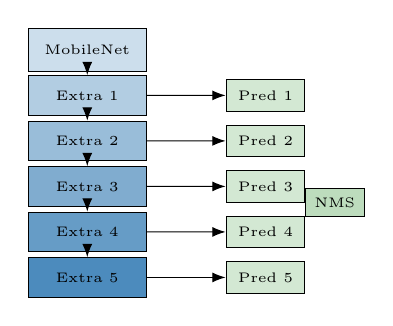
\begin{tikzpicture}[scale=0.68,every node/.style={font=\tiny}]
      \node[draw,fill=cvblue!20,minimum width=1.5cm,minimum height=0.55cm]
        (mob) at (0,4) {MobileNet};
      \foreach \i/\s/\c in {1/3.8$\times$3.8/cvblue!30,
                             2/2.6$\times$2.6/cvblue!40,
                             3/1.6$\times$1.6/cvblue!50,
                             4/0.8$\times$0.8/cvblue!60,
                             5/0.1$\times$0.1/cvblue!70}{
        \node[draw,fill=\c,minimum width=1.5cm,minimum height=0.5cm]
          (e\i) at (0,4-\i*0.85) {Extra \i};
      }
      \draw[-{Latex}] (mob)--(e1);
      \foreach \i in {1,...,4}{\pgfmathtruncatemacro{\j}{\i+1}\draw[-{Latex}](e\i)--(e\j);}
      % Prediction heads
      \foreach \i in {1,...,5}{
        \node[draw,fill=cvgreen!20,minimum width=1.0cm,minimum height=0.4cm,right=1.0cm of e\i]
          (p\i) {Pred \i};
        \draw[-{Latex}] (e\i)--(p\i);
      }
      \node[draw,fill=cvgreen!30,below=0.3cm of p3,right=0.5cm] (nms2) {NMS};
    \end{tikzpicture}
  \end{columns}
\end{frame}

% FRAME 22 — SSD Default Boxes
\begin{frame}{SSD Default Box Configuration}
  \begin{center}
  \small
  \begin{tabular}{ccccc}
    \toprule
    \textbf{Feature Map} & \textbf{Size} & \textbf{Scale} & \textbf{Aspect Ratios} & \textbf{\# Boxes}\\
    \midrule
    Conv4\_3  & $38\times38$ & 0.1   & 1, 2, 0.5              & $38^2 \times 4 = 5776$\\
    FC7       & $19\times19$ & 0.2   & 1, 2, 3, 0.5, 0.33     & $19^2 \times 6 = 2166$\\
    Conv6\_2  & $10\times10$ & 0.375 & 1, 2, 3, 0.5, 0.33     & $10^2 \times 6 = 600$\\
    Conv7\_2  & $5\times5$   & 0.55  & 1, 2, 3, 0.5, 0.33     & $5^2  \times 6 = 150$\\
    Conv8\_2  & $3\times3$   & 0.725 & 1, 2, 0.5              & $3^2  \times 4 = 36$\\
    Conv9\_2  & $1\times1$   & 0.9   & 1, 2, 0.5              & $1^2  \times 4 = 4$\\
    \midrule
    \textbf{Total} & & & & \textbf{8732}\\
    \bottomrule
  \end{tabular}
  \end{center}
  \begin{block}{Default Box Formula}
    \[
      s_k = s_{\min} + \frac{s_{\max} - s_{\min}}{m-1}(k-1), \quad k \in \{1,\ldots,m\}
    \]
    Additional scale: $s'_k = \sqrt{s_k s_{k+1}}$ for aspect ratio 1.
  \end{block}
\end{frame}

% FRAME 23 — SSD Code
\begin{frame}[fragile]{MobileNet-SSD with OpenCV DNN — Code}
\begin{lstlisting}
import cv2
import numpy as np

# Load MobileNet-SSD (Caffe format)
net    = cv2.dnn.readNetFromCaffe('deploy.prototxt',
                                   'mobilenet_iter_73000.caffemodel')
CLASSES = ["background","aeroplane","bicycle","bird","boat","bottle",
           "bus","car","cat","chair","cow","diningtable","dog","horse",
           "motorbike","person","pottedplant","sheep","sofa","train","tvmonitor"]

img = cv2.imread('street.jpg')
(H, W) = img.shape[:2]

# SSD expects 300x300, subtract mean=(127.5,127.5,127.5), scale=1/127.5
blob = cv2.dnn.blobFromImage(cv2.resize(img,(300,300)),
                              0.007843, (300,300), 127.5)
net.setInput(blob)
detections = net.forward()   # shape: (1, 1, N, 7)

for i in range(detections.shape[2]):
    confidence = detections[0,0,i,2]
    if confidence > 0.5:
        idx = int(detections[0,0,i,1])
        box = detections[0,0,i,3:7] * np.array([W,H,W,H])
        (x1,y1,x2,y2) = box.astype(int)
        cv2.rectangle(img,(x1,y1),(x2,y2),(0,255,0),2)
        label = f'{CLASSES[idx]}: {confidence:.2f}'
        cv2.putText(img, label,(x1,y1-5),
                    cv2.FONT_HERSHEY_SIMPLEX,0.5,(0,255,0),1)
\end{lstlisting}
\end{frame}

% FRAME 24 — Faster R-CNN
\begin{frame}{Faster R-CNN — Two-Stage Pipeline}
  \begin{columns}
    \column{0.52\textwidth}
    \begin{block}{Architecture (Ren et al., 2015)}
      \begin{enumerate}
        \item \textbf{Shared Backbone} (ResNet/VGG): extract feature map
        \item \textbf{Region Proposal Network}: predict $\sim$300 ROI proposals
        \item \textbf{ROI Pooling}: crop-and-resize features for each ROI to $7\times7$
        \item \textbf{Detection Head}: FC layers $\rightarrow$ class + refined bbox
      \end{enumerate}
    \end{block}
    \column{0.44\textwidth}
    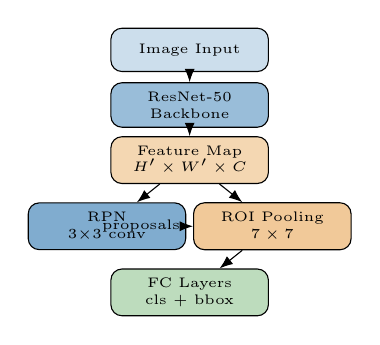
\begin{tikzpicture}[scale=0.7,every node/.style={font=\tiny},
        box/.style={draw,rounded corners,minimum width=2cm,minimum height=0.55cm,align=center}]
      \node[box,fill=cvblue!20] (inp) at (0,5)  {Image Input};
      \node[box,fill=cvblue!40] (bb)  at (0,4)  {ResNet-50\\Backbone};
      \node[box,fill=cvorange!30] (fm) at (0,3) {Feature Map\\$H'\times W'\times C$};
      \node[box,fill=cvblue!50]  (rpn) at (-1.5,1.8) {RPN\\3$\times$3 conv};
      \node[box,fill=cvorange!40](roi) at (1.5,1.8)  {ROI Pooling\\$7\times7$};
      \node[box,fill=cvgreen!30] (cls) at (0,0.6)    {FC Layers\\cls + bbox};
      \draw[-{Latex}] (inp)--(bb); \draw[-{Latex}] (bb)--(fm);
      \draw[-{Latex}] (fm)--(rpn); \draw[-{Latex}] (fm)--(roi);
      \draw[-{Latex}] (rpn)-- node[left,font=\tiny]{proposals} (roi);
      \draw[-{Latex}] (roi)--(cls);
    \end{tikzpicture}
  \end{columns}
\end{frame}

% FRAME 25 — Performance Comparison
\begin{frame}{Performance Comparison}
  \begin{center}
  \footnotesize
  \begin{tabular}{lccccc}
    \toprule
    \textbf{Model} & \textbf{mAP COCO} & \textbf{FPS (GPU)} & \textbf{FPS (CPU)} & \textbf{Size} & \textbf{Input}\\
    \midrule
    Haar Cascade        & N/A  & 30+  & 15+ & $<$1 MB  & 24$\times$24\\
    HOG+SVM             & N/A  & 5    & 2   & $<$1 MB  & 64$\times$128\\
    MobileNet-SSD v2    & 22.1 & 90   & 10  & 20 MB    & 300$\times$300\\
    YOLOv3              & 55.3 & 65   & 2   & 237 MB   & 416$\times$416\\
    YOLOv4              & 65.7 & 62   & 2   & 245 MB   & 416$\times$416\\
    YOLOv8n             & 37.3 & 120  & 8   & 6 MB     & 640$\times$640\\
    YOLOv8x             & 53.9 & 55   & 1   & 131 MB   & 640$\times$640\\
    Faster R-CNN (R50)  & 37.8 & 22   & 0.5 & 160 MB   & variable\\
    EfficientDet-D0     & 33.8 & 58   & 3   & 15 MB    & 512$\times$512\\
    \bottomrule
  \end{tabular}
  \end{center}
  \vspace{-4pt}
  \begin{alertblock}{Note}
    FPS values are approximate and hardware-dependent (GPU: RTX 3080; CPU: Intel i7-11th gen).
    mAP is COCO val2017.
  \end{alertblock}
\end{frame}

% FRAME 26 — Backend/Target Options
\begin{frame}{OpenCV DNN Backend and Target Options}
  \begin{center}
  \small
  \begin{tabular}{lll}
    \toprule
    \textbf{Backend} & \textbf{Target} & \textbf{Use Case}\\
    \midrule
    \texttt{DNN\_BACKEND\_DEFAULT}   & \texttt{DNN\_TARGET\_CPU}        & CPU inference (all platforms)\\
    \texttt{DNN\_BACKEND\_CUDA}      & \texttt{DNN\_TARGET\_CUDA}       & NVIDIA GPU (CUDA 11+)\\
    \texttt{DNN\_BACKEND\_CUDA}      & \texttt{DNN\_TARGET\_CUDA\_FP16} & NVIDIA GPU, half precision\\
    \texttt{DNN\_BACKEND\_OPENCV}    & \texttt{DNN\_TARGET\_OPENCL}     & AMD/Intel GPU via OpenCL\\
    \texttt{DNN\_BACKEND\_OPENCV}    & \texttt{DNN\_TARGET\_OPENCL\_FP16}& OpenCL half precision\\
    \texttt{DNN\_BACKEND\_INFERENCE\_ENGINE} & \texttt{DNN\_TARGET\_CPU} & Intel OpenVINO CPU\\
    \texttt{DNN\_BACKEND\_INFERENCE\_ENGINE} & \texttt{DNN\_TARGET\_MYRIAD}& Intel Myriad VPU (NCS2)\\
    \bottomrule
  \end{tabular}
  \end{center}
  \begin{columns}
    \column{0.48\textwidth}
    \begin{block}{Typical Performance Gain (YOLOv4-416)}
      \begin{itemize}
        \item CPU: $\sim$2 FPS
        \item OpenCL (Intel UHD): $\sim$8 FPS
        \item CUDA FP32: $\sim$62 FPS
        \item CUDA FP16: $\sim$90 FPS
      \end{itemize}
    \end{block}
    \column{0.48\textwidth}
    \begin{lstlisting}[basicstyle=\ttfamily\scriptsize]
net.setPreferableBackend(
    cv2.dnn.DNN_BACKEND_CUDA)
net.setPreferableTarget(
    cv2.dnn.DNN_TARGET_CUDA_FP16)
    \end{lstlisting}
  \end{columns}
\end{frame}

% ============================================================
% PART 4 — CUSTOM TRAINING
% ============================================================

% FRAME 27 — Dataset Preparation
\begin{frame}{Dataset Preparation Workflow}
  \begin{center}
  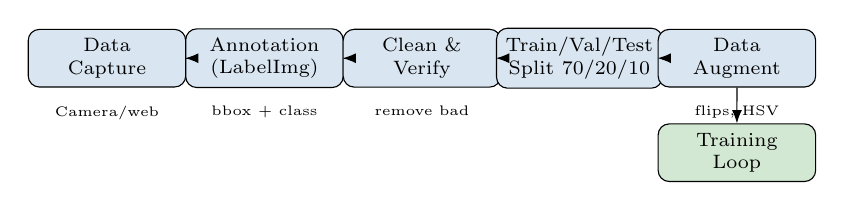
\begin{tikzpicture}[scale=0.8,every node/.style={font=\scriptsize},
      box/.style={draw,rounded corners,fill=cvblue!15,minimum width=2cm,minimum height=0.7cm,align=center}]
    \node[box] (cap)  at (0,0)    {Data\\Capture};
    \node[box] (ann)  at (2.5,0)  {Annotation\\(LabelImg)};
    \node[box] (cln)  at (5,0)    {Clean \&\\Verify};
    \node[box] (spl)  at (7.5,0)  {Train/Val/Test\\Split 70/20/10};
    \node[box] (aug)  at (10,0)   {Data\\Augment};
    \node[box,fill=cvgreen!20] (trn) at (10,-1.5) {Training\\Loop};
    \foreach \a/\b in {cap/ann,ann/cln,cln/spl,spl/aug,aug/trn}{\draw[-{Latex}](\a)--(\b);}
    % Sub-labels
    \node[font=\tiny,below=3pt of cap] {Camera/web};
    \node[font=\tiny,below=3pt of ann] {bbox + class};
    \node[font=\tiny,below=3pt of cln] {remove bad};
    \node[font=\tiny,below=3pt of aug] {flips, HSV};
  \end{tikzpicture}
  \end{center}
  \begin{block}{Recommended Tools}
    \begin{itemize}
      \item \textbf{LabelImg} / \textbf{Roboflow Annotate} / \textbf{CVAT} — bounding box annotation
      \item \textbf{Roboflow} — dataset versioning, augmentation pipeline, export to YOLO/COCO
      \item \textbf{FiftyOne} — dataset visualisation and cleaning
    \end{itemize}
  \end{block}
\end{frame}

% FRAME 28 — Annotation Formats
\begin{frame}[fragile]{Annotation Format Comparison}
  \begin{columns}
    \column{0.32\textwidth}
    \begin{block}{YOLO TXT}
\begin{lstlisting}
# class cx cy w h
# (normalised 0-1)
0 0.5 0.4 0.2 0.3
1 0.7 0.6 0.1 0.2
\end{lstlisting}
    One \texttt{.txt} per image\\
    Same filename as image
    \end{block}
    \column{0.32\textwidth}
    \begin{block}{COCO JSON}
\begin{lstlisting}
{"annotations": [{
  "id": 1,
  "image_id": 42,
  "category_id": 1,
  "bbox": [x,y,w,h],
  "area": 1200,
  "iscrowd": 0
}]}
\end{lstlisting}
    Single JSON for all images
    \end{block}
    \column{0.32\textwidth}
    \begin{block}{Pascal VOC XML}
\begin{lstlisting}
<annotation>
 <object>
  <name>cat</name>
  <bndbox>
   <xmin>100</xmin>
   <ymin>80</ymin>
   <xmax>200</xmax>
   <ymax>250</ymax>
  </bndbox>
 </object>
</annotation>
\end{lstlisting}
    One XML per image
    \end{block}
  \end{columns}
\end{frame}

% FRAME 29 — YOLOv8 Training Hyperparameters
\begin{frame}{YOLOv8 Training — Key Hyperparameters}
  \begin{center}
  \footnotesize
  \begin{tabular}{lllp{5cm}}
    \toprule
    \textbf{Param} & \textbf{Default} & \textbf{Range} & \textbf{Description}\\
    \midrule
    \texttt{imgsz}   & 640    & 320--1280  & Input image size (square)\\
    \texttt{batch}   & 16     & 1--64      & Batch size; -1 = auto\\
    \texttt{epochs}  & 100    & 10--1000   & Training epochs\\
    \texttt{lr0}     & 0.01   & 0.001--0.1 & Initial learning rate\\
    \texttt{lrf}     & 0.01   & 0.001--0.1 & Final LR = lr0 * lrf\\
    \texttt{momentum}& 0.937  & 0.6--0.98  & SGD momentum\\
    \texttt{weight\_decay} & 0.0005 & 0--0.01 & L2 regularisation\\
    \texttt{warmup\_epochs} & 3.0 & 0--10  & LR warmup epochs\\
    \texttt{mosaic}  & 1.0    & 0.0--1.0   & Mosaic augmentation prob.\\
    \texttt{mixup}   & 0.0    & 0.0--1.0   & MixUp augmentation prob.\\
    \texttt{degrees} & 0.0    & 0--180     & Rotation augmentation\\
    \texttt{hsv\_h}  & 0.015  & 0--1       & HSV hue augmentation\\
    \texttt{patience}& 50     & 0--300     & Early stopping patience\\
    \bottomrule
  \end{tabular}
  \end{center}
\end{frame}

% FRAME 30 — Transfer Learning
\begin{frame}{Transfer Learning for Custom Detection}
  \begin{center}
  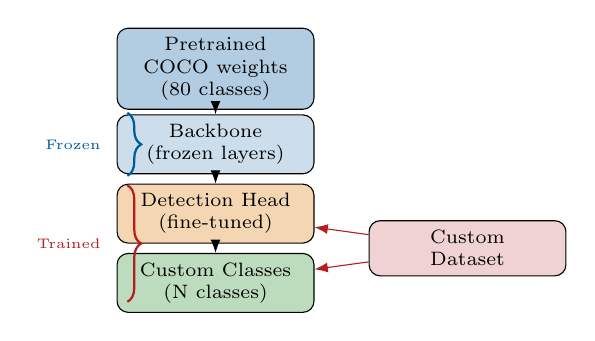
\begin{tikzpicture}[scale=0.8,every node/.style={font=\scriptsize},
      box/.style={draw,rounded corners,minimum width=2.5cm,minimum height=0.7cm,align=center}]
    % Pretrained
    \node[box,fill=cvblue!30] (pre)  at (0,3)   {Pretrained\\COCO weights\\(80 classes)};
    \node[box,fill=cvblue!20] (bb)   at (0,1.8) {Backbone\\(frozen layers)};
    \node[box,fill=cvorange!30](head) at (0,0.7) {Detection Head\\(fine-tuned)};
    \node[box,fill=cvgreen!30] (out)  at (0,-0.4){Custom Classes\\(N classes)};
    \draw[-{Latex}] (pre)--(bb);
    \draw[-{Latex}] (bb)--(head);
    \draw[-{Latex}] (head)--(out);
    % Freeze annotation
    \draw[cvblue,thick,decorate,decoration={brace,amplitude=5pt}]
         (-1.4,2.3)--(-1.4,1.3) node[midway,left=6pt,font=\tiny,cvblue]{Frozen};
    \draw[cvred,thick,decorate,decoration={brace,amplitude=5pt}]
         (-1.4,1.15)--(-1.4,-0.7) node[midway,left=6pt,font=\tiny,cvred]{Trained};
    % Arrow from custom data
    \node[box,fill=cvred!20] (data) at (4,0.15) {Custom\\Dataset};
    \draw[-{Latex},cvred] (data)--(head);
    \draw[-{Latex},cvred] (data)--(out);
  \end{tikzpicture}
  \end{center}
  \begin{lstlisting}[basicstyle=\ttfamily\scriptsize]
from ultralytics import YOLO
model = YOLO('yolov8n.pt')                    # load COCO pretrained
results = model.train(data='custom.yaml',
                      epochs=100, imgsz=640,
                      freeze=10)               # freeze first 10 backbone layers
  \end{lstlisting}
\end{frame}

% FRAME 31 — ONNX Export
\begin{frame}[fragile]{ONNX Export for OpenCV Inference}
  \begin{lstlisting}
from ultralytics import YOLO

model = YOLO('runs/detect/train/weights/best.pt')

# Export to ONNX (opset 12 for OpenCV DNN compatibility)
model.export(format='onnx', opset=12,
             simplify=True,     # run onnx-simplifier
             dynamic=False,     # static batch size
             imgsz=640)

# Verify exported model
import onnx
m = onnx.load('best.onnx')
onnx.checker.check_model(m)
print(f'ONNX opset: {m.opset_import[0].version}')
# Output shape: [1, 4+num_classes, 8400]
  \end{lstlisting}
  \begin{block}{ONNX Compatibility Notes}
    \begin{itemize}
      \item Use \texttt{opset=12} for OpenCV 4.7+ DNN module
      \item Set \texttt{dynamic=False} to fix batch/size for DNN
      \item Run \texttt{onnxsim} to fold constants and remove unused nodes
      \item OpenVINO users: convert to IR format for extra performance
    \end{itemize}
  \end{block}
\end{frame}

% FRAME 32 — YOLOv8 ONNX Inference in OpenCV
\begin{frame}[fragile]{YOLOv8 ONNX Inference in OpenCV DNN}
\begin{lstlisting}
import cv2, numpy as np

net = cv2.dnn.readNetFromONNX('best.onnx')
net.setPreferableBackend(cv2.dnn.DNN_BACKEND_CUDA)
net.setPreferableTarget(cv2.dnn.DNN_TARGET_CUDA)

img = cv2.imread('test.jpg')
H, W = img.shape[:2]
blob = cv2.dnn.blobFromImage(img, 1/255.0, (640,640), swapRB=True, crop=False)
net.setInput(blob)
pred = net.forward()[0]   # shape: [4+num_classes, 8400]

# Transpose to [8400, 4+num_classes]
pred = pred.T
boxes, scores, class_ids = [], [], []
for row in pred:
    cls_scores = row[4:]
    cid = np.argmax(cls_scores)
    conf = cls_scores[cid]
    if conf < 0.5: continue
    cx, cy, w, h = row[:4]
    # Scale to original image
    x1 = int((cx - w/2) * W/640)
    y1 = int((cy - h/2) * H/640)
    x2 = int((cx + w/2) * W/640)
    y2 = int((cy + h/2) * H/640)
    boxes.append([x1, y1, x2-x1, y2-y1])
    scores.append(float(conf))
    class_ids.append(cid)

idx = cv2.dnn.NMSBoxes(boxes, scores, 0.5, 0.45)
for i in idx.flatten():
    x,y,w,h = boxes[i]
    cv2.rectangle(img,(x,y),(x+w,y+h),(0,255,0),2)
\end{lstlisting}
\end{frame}

% FRAME 33 — HOG+SVM Custom Training
\begin{frame}[fragile]{HOG+SVM Custom Training}
\begin{lstlisting}
import cv2, numpy as np
from sklearn.svm import SVC
from sklearn.preprocessing import StandardScaler

hog = cv2.HOGDescriptor((64,128), (16,16), (8,8), (8,8), 9)

def extract(img):
    img = cv2.resize(img, (64,128))
    gray = cv2.cvtColor(img, cv2.COLOR_BGR2GRAY)
    return hog.compute(gray).flatten()

# Build feature matrix
pos_images = [...]   # list of positive sample images
neg_images = [...]   # list of negative sample images
X = np.array([extract(i) for i in pos_images + neg_images])
y = np.array([1]*len(pos_images) + [0]*len(neg_images))

# Train SVM
scaler = StandardScaler()
X_scaled = scaler.fit_transform(X)
svm = SVC(kernel='rbf', C=1.0, probability=True)
svm.fit(X_scaled, y)

# For OpenCV HOGDescriptor setSVMDetector, need linear SVM coefficients
from sklearn.svm import LinearSVC
lin_svm = LinearSVC(C=0.01, max_iter=2000)
lin_svm.fit(X_scaled, y)

sv = lin_svm.coef_[0]
b  = lin_svm.intercept_[0]
detector = np.append(sv, -b).astype(np.float32)
hog.setSVMDetector(detector)
\end{lstlisting}
\end{frame}

% FRAME 34 — Evaluation Metrics
\begin{frame}{Evaluation Metrics: Precision, Recall, mAP}
  \begin{columns}
    \column{0.45\textwidth}
    \begin{block}{Definitions}
      \[
        P = \frac{TP}{TP+FP}, \quad R = \frac{TP}{TP+FN}
      \]
      \[
        AP = \int_0^1 P(R)\,dR \approx \sum_k P_k \Delta R_k
      \]
      \[
        \text{mAP} = \frac{1}{C}\sum_{c=1}^{C} AP_c
      \]
      COCO mAP = mean over IoU $\in [0.5:0.05:0.95]$
    \end{block}
    \column{0.52\textwidth}
    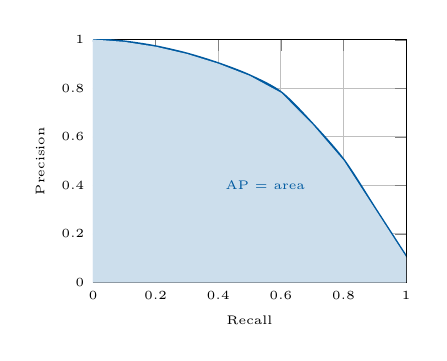
\begin{tikzpicture}[scale=0.9]
      \begin{axis}[
        xlabel=Recall,ylabel=Precision,
        xmin=0,xmax=1,ymin=0,ymax=1,
        width=6cm,height=5cm,
        grid=major,
        tick label style={font=\tiny},
        label style={font=\tiny}]
        % PR curve
        \addplot[cvblue,ultra thick,smooth] coordinates {
          (0,1.0)(0.1,0.99)(0.2,0.97)(0.3,0.94)(0.4,0.90)
          (0.5,0.85)(0.6,0.78)(0.7,0.65)(0.8,0.50)(0.9,0.30)(1.0,0.1)};
        % Shaded area
        \addplot[cvblue!20,fill=cvblue!20] coordinates {
          (0,1.0)(0.1,0.99)(0.2,0.97)(0.3,0.94)(0.4,0.90)
          (0.5,0.85)(0.6,0.78)(0.7,0.65)(0.8,0.50)(0.9,0.30)(1.0,0.1)
          (1.0,0)(0,0)} \closedcycle;
        \node[font=\tiny,cvblue] at (axis cs:0.55,0.4) {AP = area};
      \end{axis}
    \end{tikzpicture}
  \end{columns}
\end{frame}

% ============================================================
% PART 5 — ADVANCED TOPICS
% ============================================================

% FRAME 35 — Multi-Scale Detection Pyramid
\begin{frame}{Multi-Scale Detection — Feature Pyramid}
  \begin{center}
  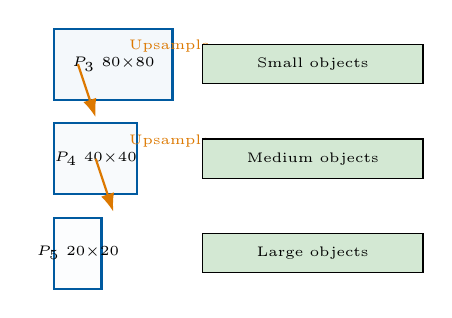
\begin{tikzpicture}[scale=0.75,every node/.style={font=\tiny}]
    % Bottom-up pathway (encoder)
    \foreach \i/\l/\s in {0/$P_5$ 20$\times$20/0.8, 1.6/$P_4$ 40$\times$40/1.4, 3.2/$P_3$ 80$\times$80/2.0}{
      \pgfmathparse{int(\i*10+5)}
      \draw[fill=cvblue!\pgfmathresult!white,draw=cvblue,thick]
           (0,\i) rectangle (\s,\i+1.2);
      \node at (\s/2,\i+0.6) {\l};
    }
    % Top-down pathway (decoder)
    \draw[-{Latex},cvorange,thick] (0.8/2,3.2+0.6) -- (1.4/2,1.6+1.3);
    \draw[-{Latex},cvorange,thick] (1.4/2,1.6+0.6) -- (2.0/2,0.0+1.3);
    \node[cvorange,right] at (1.1,4.1) {Upsample};
    \node[cvorange,right] at (1.1,2.5) {Upsample};
    % Detection heads
    \foreach \i/\obj in {0/Large objects, 1.6/Medium objects, 3.2/Small objects}{
      \node[draw,fill=cvgreen!20,right=0.3cm,minimum width=2.8cm,minimum height=0.5cm]
            at (2.1,\i+0.6) {\obj};
    }
  \end{tikzpicture}
  \end{center}
  \begin{block}{Why Multi-Scale?}
    Small feature maps (large stride) capture \textbf{semantic context} for large objects.
    Large feature maps (small stride) retain \textbf{spatial resolution} for small objects.
    FPN merges both via lateral connections.
  \end{block}
\end{frame}

% FRAME 36 — Data Augmentation
\begin{frame}{Data Augmentation Strategies for Detection}
  \begin{columns}
    \column{0.48\textwidth}
    \begin{block}{Geometric Augmentations}
      \begin{itemize}
        \item \textbf{Horizontal flip}: $p=0.5$
        \item \textbf{Random crop}: maintain $\geq 0.4$ IoU with GT
        \item \textbf{Scale jitter}: $[0.5\times, 2.0\times]$
        \item \textbf{Rotation}: $\pm 10°$ (careful: bbox must follow)
        \item \textbf{Perspective warp}: subtle distortion
      \end{itemize}
    \end{block}
    \begin{block}{Colour Augmentations}
      \begin{itemize}
        \item HSV shift: \texttt{hsv\_h=0.015, hsv\_s=0.7, hsv\_v=0.4}
        \item Brightness / contrast jitter
        \item Random grayscale conversion
      \end{itemize}
    \end{block}
    \column{0.48\textwidth}
    \begin{block}{Advanced Mixing Strategies}
      \begin{itemize}
        \item \textbf{Mosaic} (YOLO): 4 images tiled into one; forces learning of partial objects
        \item \textbf{MixUp}: blend two images $\tilde{x} = \lambda x_1 + (1-\lambda)x_2$
        \item \textbf{CutMix}: paste random patch from $x_2$ onto $x_1$
        \item \textbf{Copy-Paste}: copy object instances from other images
      \end{itemize}
    \end{block}
    \vspace{2pt}
    \begin{alertblock}{Tip}
      Always augment \textbf{both image and bounding boxes} together!
    \end{alertblock}
  \end{columns}
\end{frame}

% FRAME 37 — Tracking Integration
\begin{frame}[fragile]{Tracking Integration After Detection}
  \begin{columns}
    \column{0.52\textwidth}
    \begin{block}{Detect-then-Track Pipeline}
      \begin{enumerate}
        \item Run detector every $N$ frames to initialise/update trackers
        \item Between frames: propagate trackers cheaply
        \item Re-detect when tracker confidence drops
      \end{enumerate}
    \end{block}
    \small
    \begin{tabular}{lll}
      \toprule
      \textbf{Tracker} & \textbf{Speed} & \textbf{Accuracy}\\
      \midrule
      MOSSE & Very fast & Low\\
      KCF   & Fast      & Medium\\
      CSRT  & Medium    & High\\
      \bottomrule
    \end{tabular}
    \column{0.44\textwidth}
    \begin{lstlisting}
import cv2
tracker = cv2.TrackerCSRT_create()

cap = cv2.VideoCapture(0)
ret, frame = cap.read()

# Initialise from detection bbox
bbox = (x, y, w, h)
tracker.init(frame, bbox)

while True:
    ret, frame = cap.read()
    ok, bbox = tracker.update(frame)
    if ok:
        x,y,w,h = [int(v) for v in bbox]
        cv2.rectangle(frame,
          (x,y),(x+w,y+h),
          (0,255,0), 2)
    cv2.imshow('Track', frame)
    if cv2.waitKey(1) == 27: break
    \end{lstlisting}
  \end{columns}
\end{frame}

% FRAME 38 — Edge Deployment
\begin{frame}{Edge Deployment — Quantisation and Optimisation}
  \begin{columns}
    \column{0.48\textwidth}
    \begin{block}{Model Quantisation}
      \begin{itemize}
        \item \textbf{FP32} $\rightarrow$ \textbf{FP16}: $2\times$ smaller, minimal accuracy loss
        \item \textbf{FP32} $\rightarrow$ \textbf{INT8}: $4\times$ smaller, $2{-}4\times$ faster, 1--2\% AP drop
        \item Post-Training Quantisation (PTQ): calibration data only
        \item Quantisation-Aware Training (QAT): re-train with fake quantisation
      \end{itemize}
    \end{block}
    \column{0.48\textwidth}
    \begin{block}{Deployment Stacks}
      \begin{itemize}
        \item \textbf{ONNX Runtime} + INT8: Jetson Nano, RPi
        \item \textbf{TensorRT} (NVIDIA): best GPU performance
        \item \textbf{OpenVINO} (Intel): Myriad, Core, Atom
        \item \textbf{TFLite}: Android, Coral Edge TPU
        \item \textbf{NCNN} (Tencent): ARM mobile, no deps
      \end{itemize}
    \end{block}
  \end{columns}
  \begin{lstlisting}[basicstyle=\ttfamily\scriptsize]
# Export YOLOv8 to INT8 ONNX via TensorRT
from ultralytics import YOLO
model = YOLO('best.pt')
model.export(format='engine', int8=True,     # TensorRT INT8
             data='calibration.yaml', batch=1)
  \end{lstlisting}
\end{frame}

% FRAME 39 — Decision Flowchart
\begin{frame}{Which Method to Choose? — Decision Guide}
  \begin{center}
  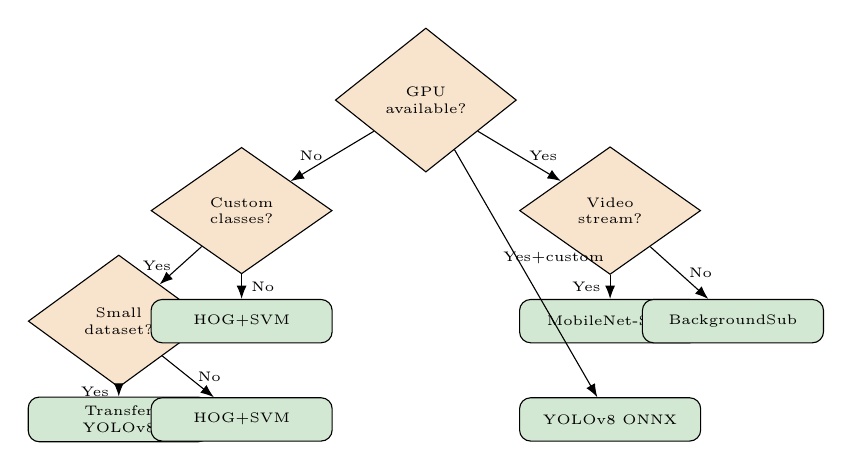
\begin{tikzpicture}[scale=0.78,every node/.style={font=\tiny},
      dec/.style={diamond,draw,fill=cvorange!20,align=center,
                  minimum width=2.3cm,minimum height=0.7cm},
      res/.style={draw,rounded corners,fill=cvgreen!20,align=center,
                  minimum width=2.3cm,minimum height=0.55cm}]
    \node[dec] (gpu) at (0,0)     {GPU\\available?};
    \node[dec] (cst) at (-3,-1.8) {Custom\\classes?};
    \node[dec] (vid) at (3,-1.8)  {Video\\stream?};
    \node[dec] (sml) at (-5,-3.6) {Small\\dataset?};
    \node[res] (hogr)at (-3,-3.6) {HOG+SVM};
    \node[res] (ssd) at (3,-3.6)  {MobileNet-SSD};
    \node[res] (bg)  at (5,-3.6)  {BackgroundSub};
    \node[res] (yt)  at (-5,-5.2) {Transfer\\YOLOv8};
    \node[res] (hog2)at (-3,-5.2) {HOG+SVM};
    \node[res] (yolo)at (3,-5.2)  {YOLOv8 ONNX};
    \draw[-{Latex}] (gpu) -- node[left]{No}  (cst);
    \draw[-{Latex}] (gpu) -- node[right]{Yes} (vid);
    \draw[-{Latex}] (cst) -- node[left]{Yes} (sml);
    \draw[-{Latex}] (cst) -- node[right]{No}  (hogr);
    \draw[-{Latex}] (vid) -- node[left]{Yes}  (ssd);
    \draw[-{Latex}] (vid) -- node[right]{No}  (bg);
    \draw[-{Latex}] (sml) -- node[left]{Yes}  (yt);
    \draw[-{Latex}] (sml) -- node[right]{No}  (hog2);
    \draw[-{Latex}] (gpu) -- node[above,xshift=10pt]{Yes+custom} (yolo);
  \end{tikzpicture}
  \end{center}
\end{frame}

% ============================================================
% FRAME 40 — References
% ============================================================
\begin{frame}{References and Further Reading}
  \begin{thebibliography}{9}
    \setbeamertemplate{bibliography item}[text]
    \bibitem{vj2001}
      P.~Viola and M.~Jones, ``Rapid Object Detection using a Boosted Cascade of Simple Features,''
      \emph{CVPR}, 2001.
    \bibitem{dt2005}
      N.~Dalal and B.~Triggs, ``Histograms of Oriented Gradients for Human Detection,''
      \emph{CVPR}, 2005.
    \bibitem{yolo2016}
      J.~Redmon et al., ``You Only Look Once: Unified, Real-Time Object Detection,''
      \emph{CVPR}, 2016.
    \bibitem{ssd2016}
      W.~Liu et al., ``SSD: Single Shot MultiBox Detector,''
      \emph{ECCV}, 2016.
    \bibitem{frcnn2015}
      S.~Ren et al., ``Faster R-CNN: Towards Real-Time Object Detection with Region Proposal Networks,''
      \emph{NeurIPS}, 2015.
    \bibitem{yolov8}
      G.~Jocher et al., ``Ultralytics YOLOv8,'' \url{https://github.com/ultralytics/ultralytics}, 2023.
    \bibitem{opencv}
      OpenCV DNN module documentation: \url{https://docs.opencv.org/master/d6/d0f/group__dnn.html}
  \end{thebibliography}
  \vspace{6pt}
  \begin{center}
    \large\textbf{Thank you!} \\[4pt]
    \small Full code examples at \texttt{opencv.org/docs}
  \end{center}
\end{frame}

\end{document}
